%%%%%%%%%%%%%%%%%%%%%%%%%%%%%%%%%%%%%%%%%%%%%%%%%%%%%%%%%%%%%%%%%%%%%%
% Colorado State University LaTeX Thesis Template and Documentation
%
% by
%   Elliott Forney
%
% This is free and unencumbered software released into the public domain.
% 
% Anyone is free to copy, modify, publish, use, compile, sell, or
% distribute this software, either in source code form or as a compiled
% binary, for any purpose, commercial or non-commercial, and by any
% means.
% 
% In jurisdictions that recognize copyright laws, the author or authors
% of this software dedicate any and all copyright interest in the
% software to the public domain. We make this dedication for the benefit
% of the public at large and to the detriment of our heirs and
% successors. We intend this dedication to be an overt act of
% relinquishment in perpetuity of all present and future rights to this
% software under copyright law.
% 
% THE SOFTWARE IS PROVIDED "AS IS", WITHOUT WARRANTY OF ANY KIND,
% EXPRESS OR IMPLIED, INCLUDING BUT NOT LIMITED TO THE WARRANTIES OF
% MERCHANTABILITY, FITNESS FOR A PARTICULAR PURPOSE AND NONINFRINGEMENT.
% IN NO EVENT SHALL THE AUTHORS BE LIABLE FOR ANY CLAIM, DAMAGES OR
% OTHER LIABILITY, WHETHER IN AN ACTION OF CONTRACT, TORT OR OTHERWISE,
% ARISING FROM, OUT OF OR IN CONNECTION WITH THE SOFTWARE OR THE USE OR
% OTHER DEALINGS IN THE SOFTWARE.
%%%%%%%%%%%%%%%%%%%%%%%%%%%%%%%%%%%%%%%%%%%%%%%%%%%%%%%%%%%%%%%%%%%%%%

% Preamble
%%%%%%%%%%%%%%%%%%%%%%%%%%%%%%%%%%%%%%%%%%%%%%%%%%%%%%%%%%%%%%%%

% use the thesis document class
% this is derived from the standard book class
% and supports many of the same features
\documentclass[master]{thesis}
%\documentclass[doctor]{thesis} % for a dissertation

% fonts
% use times font by default but can specify other fonts
%\usepackage{fourier} % fourier is also a nice choice

%\usepackage[scaled]{helvet} % or these two lines give a sans-serif font
%\renewcommand\familydefault{\sfdefault} 

% this is useful for including dummy test
% it can be removed in final document
\usepackage{lipsum}

% ams math packages
\usepackage[cmex10]{amsmath}
\usepackage{amsthm,amssymb}

% graphics packages
\usepackage[pdftex]{graphicx} % remove pdftex if you are not compiling to pdf
\graphicspath{{./figures/}} % this places all graphics in the figures subdirectory

% allowed graphics extensions
% uncomment if you prefer to add extension in \includegraphics
\DeclareGraphicsExtensions{.pdf,.png,.jpg}

% allows the creation of subfigures
\usepackage[caption=false]{subfig}

% book tables are simple and look nice
\usepackage{booktabs}

% for specifying urls and links
\usepackage{url}
\urlstyle{same} % same style as regular text

% Title Page
%%%%%%%%%%%%%%%%%%%%%%%%%%%%%%%%%%%%%%%%%%%%%%%%%%%%%%%%%%%%%%%%

% title of your thesis
\title{Colorado State University LaTeX Thesis Template}

% author's name
\author{John M. Doe}

% author's email address
\email{youremail@whereever.com}

% department name
\department{Department of Computer Science}

% semester of completion
\semester{Spring 2015}

% committee member names
\advisor{Advisor Name}
\coadvisor{Co-Adivisor Name} % co-advisor is optional
\committee{First Member} % as many committee entries as you need
\committee{Second Member}
\committee{Third Member}

% Copyright Page
%%%%%%%%%%%%%%%%%%%%%%%%%%%%%%%%%%%%%%%%%%%%%%%%%%%%%%%%%%%%%%%%

% here is an example of student copyright declaration
% note that the \copyright command prints the copyright symbol,
% so we use the name \mycopyright instead
\mycopyright{%
Copyright by John M. Doe 20\_\_ \\
All Rights reserved
}

% here is an example of a creative commons copyright license
% ask the graduate school for more information
%\mycopyright{%
%This work is licensed under the Creative Commons Attribution-NonCommercial-NoDerivatives 3.0 United States License.
%
%\vspace{3em}
%
%To view a copy of this license, visit:
%
%\vspace{2em}
%
%\url{http://creativecommons.org/licenses/by-nc-nd/3.0/legalcode}
%
%\vspace{3em}
%
%Or send a letter to:
%
%\vspace{2em}
%
%Creative Commons
%
%171 Second Street, Suite 300
%
%San Francisco, California, 94105, USA.
%}

% Abstract
%%%%%%%%%%%%%%%%%%%%%%%%%%%%%%%%%%%%%%%%%%%%%%%%%%%%%%%%%%%%%%%%

\abstract{%
This document aims to get you started typesetting your thesis or dissertation in \LaTeX{}.  It serves both as a sample and as the documentation for this package.  Please review the entire document for helpful tips about formatting your thesis or dissertation.  You may replace this text with your abstract.
}

% Acknowledgments 
%%%%%%%%%%%%%%%%%%%%%%%%%%%%%%%%%%%%%%%%%%%%%%%%%%%%%%%%%%%%%%%%

\acknowledgements{%
I would like to thank the CSU Graduate Student Council for iniaiting and supporting the creation of this project and the CSU Graduate School for their assistance and feedback.  Thank you to CSU for being awsome, to the creators of \LaTeX{} for making a great typesetting tool and to everyone who has contributed to this template.  You may replace this text with your own acknowledgements.
}

% Metadata
%%%%%%%%%%%%%%%%%%%%%%%%%%%%%%%%%%%%%%%%%%%%%%%%%%%%%%%%%%%%%%%%%%%%%%

% consider using hyperref to insert pdf metadata and make links clickable
% safe to remove if not using pdf or if it causes problems
\usepackage[pdfpagelabels,pdfusetitle,colorlinks=false,pdfborder={0 0 0}]{hyperref}

\begin{document} % preamble is complete, add any custom packages above
%%%%%%%%%%%%%%%%%%%%%%%%%%%%%%%%%%%%%%%%%%%%%%%%%%%%%%%%%%%%%%%%

\frontmatter % starts preliminary pages
%%%%%%%%%%%%%%%%%%%%%%%%%%%%%%%%%%%%%%%%%%%%%%%%%%%%%%%%%%%%%%%%

\maketitle
\makemycopyright
\makeabstract
\makeacknowledgements

% any extra preliminary pages can be added here
% below is an example of a dedication page
% the dedication page is optional
\prelimtocentry{Dedication} % add table of contents entry
\begin{flatcenter} % center without extra space

    % page title
    DEDICATION

    %\vspace{3em} % place at top
    \vfill % or center on page

    \noindent \textit{I would like to dedicate this thesis to my dog fluffy.}
    \vfill % fill extra space at bottom
\end{flatcenter}
\newpage

\tableofcontents
\listoftables % optional
\listoffigures % optional

\mainmatter % starts thesis body
%%%%%%%%%%%%%%%%%%%%%%%%%%%%%%%%%%%%%%%%%%%%%%%%%%%%%%%%%%%%%%%%

\chapter{Introduction}
\label{chap:intro}
%%%%%%%%%%%%%%%%%%%%%%%%%%%%%%%%%%%%%%%%%%%%%%%%%%%%%%%%%%%%%%%%

Thank you for downloading the Colorado State University (CSU) \LaTeX{} document class and template for theses and dissertations.  The goal of this document is to get you started writing and typesetting your thesis in \LaTeX{}.  This document serves both as a guide for using this package and as a sample template to get you started.  Please review the entire document for useful information on typesetting your thesis or dissertation.  After reading over this guide, please see the source code for this document to get started.

Please note that while this package was sponsored by the CSU Graduate Student Council and by the CSU Graduate School, it is not officially supported by CSU.  Instead, it is intended that this document will be supported by its community of users and by the students themselves, that's you!  This document is currently hosted on GitHub at \url{https://github.com/idfah/csuthesis}.  If you have a patch or improvement that you would like included, please submit a pull request on GitHub.  For information on the official guidelines for formatting your thesis, please visit the CSU electronic thesis and dissertation resources page at \url{http://graduateschool.colostate.edu/for-current-students/completing-your-degree/thesis-dissertation/}.

Also, note that this package is free software.  See the header of the source code for the full copyright license.  You are free to modify, distribute, fork and otherwise use this software in any that you would like.

\chapter{The Thesis Document Class}

This package includes a \LaTeX{} document class called \textit{thesis.cls}, which extends the \textit{book.cls} that is included with standard \LaTeX{} distributions.  Many of the features that work in \textit{book.cls} will also work in \textit{thesis.cls}; however, the setup of the title and other preliminary pages and various aspects of the document's formatting have been modified.  Note that \textit{thesis.cls} passes the following options to \textit{book.cls}: \textbf{oneside}, \textbf{openany}, \textbf{letterpaper}, \textbf{12pt}.  This means that your thesis will have a 12pt font and does not leave extra space on odd pages for binding.  Also, \textit{thesis.cls} provides a few extra options and commands that may be useful.  These features are described in detail below.

\section{Required Packages}

You will need to have several \LaTeX{} packages installed in order for \textit{thesis.cls} to work correctly.  While most standard \LaTeX{} distributions include these packages, some systems may require you to install them.  In Linux with texlive, For example, you may need to locate some of these packages (they are typically called something like texlive-packagename).

\begin{itemize}
    \item \textbf{geometry}  This package is required for setting up your document's margins.

    \item \textbf{setspace}  This package is required to enable double spacing.

    \item \textbf{pdflscape}  or \textbf{lscape}  These packages are required for inserting landscape pages.  \textbf{pdflscape} is required if you are compiling directly to pdf (using the pdf class option described below) and \textbf{lscape} is required if you are not compiling to pdf.

    \item \textbf{fontenc} and \textbf{times}  These packages are required for setting up the default \textit{times} font.  Note that you may use a different font, if you choose, by loading the corresponding package after loading the document class.

    \item \textbf{footmisc}  This package is required for setting up footnotes.

    \item \textbf{remreset}  This package is required for preventing the footnote numbering from resetting after each chapter.

    \item \textbf{caption}  This package is required for formatting captions around figures and tables.

    \item \textbf{tocloft}  This package is required for formatting the table of contents and similar pages.

    \item \textbf{cite}  This package is required for citing various things, including tables figures and references.
\end{itemize}

\section{Document Class Options}

The \textit{thesis.cls} document class also provides a number of options that can be specified when the class is loaded.  The following class options are supported:

\begin{itemize}
    \item \textbf{bachelor}  This sets the formatting style to be suitable for an undergraduate Honor's Thesis.

    \item \textbf{master}  This sets the formatting style to be appropriate for a graduate Master's Thesis.

    \item \textbf{doctor}  This sets the formatting style to be appropriate for a graduate PhD Dissertation.

    \item \textbf{showframe}  This shows a frame around the page at the margins, headers and footers.  This can be useful for debugging problems with your margins, e.g., if your top margin is too large.

    \item \textbf{raggedright}  This options formats your document with left-justified text and a ragged right margin.   Without setting this option, the standard fully-justified format will be used and words will be hyphenated when necessary for line breaks.  Note that \textbf{raggedright} looks more like an MS Word document while the default looks more like a typical \LaTeX{} document.

    \item \textbf{nopdf}  This prevents the use of features that are specific to pdf output formats.  Specify this option if you are using a different format, such as PostScript or DVI.

    \item \textbf{subfigure}  This enables compatibility with the \textit{subfigure} package.  Note that \textit{subfigure} is now depreciated in favor of the \textit{subfig} package, which is supported by default.
\end{itemize}

In addition to the above options, \textit{thesis.cls} supports all of the options supported by \textit{book.cls}.  We recommend, however, that you double check the Graduate School's formatting guidelines before changing any of the options from \textit{book.cls}.

\section{Preliminary Pages}

A number of commands are provided by \textit{thesis.cls} to create the various preliminary pages that must be included in your thesis, e.g, title page, copyright page, abstract, table of contents, et cetra.  The following commands provide information to \textit{thesis.cls} about the contents of your preliminary pages and should be specified before \verb|\begin{document}|.

\begin{itemize}
    \item \textbf{\textbackslash title}  This command takes a single argument giving the title of your thesis.
    \item \textbf{\textbackslash author}  This command takes a single argument giving the name of the author.
    \item \textbf{\textbackslash email}  This command takes a single argument giving the author's email address.
    \item \textbf{\textbackslash department}  This command takes a single argument giving the name of the author's department, e.g., Department of Computer Science.
    \item \textbf{\textbackslash semester}  This command takes a single argument giving the semester during which the thesis will be defended, e.g., Summer 2017.
    \item \textbf{\textbackslash advisor}  This command takes a single argument giving the name of the author's advisor, do not include Dr. or Professor.
    \item \textbf{\textbackslash coadvisor}  This is an optional command that takes a single argument specifying the author's co-advisor.  Omit this command if you don't have a co-advisor.
    \item \textbf{\textbackslash committee}  This command takes a single argument giving the name of a member of the author's committee.  Use this command repeatedly to specify additional committee members.
    \item \textbf{\textbackslash mycopyright}  This command takes a single argument giving the text to display on the copyright page.  Ask the graduate school for more information on choosing the copyright that is right for you.
    \item \textbf{\textbackslash abstract}  This command takes a single argument giving the text to display on the abstract page.
    \item \textbf{\textbackslash acknowledgements}  This command takes a single argument giving the text to display on the acknowledgements page.
\end{itemize}

After you have finished your preamble and specified \verb|\begin{document}|, the following commands can be used to actually insert each preliminary page:

\begin{itemize}
    \item \textbf{\textbackslash maketitle}  Makes the title page.
    \item \textbf{\textbackslash makemycopyright}  Makes the copyright page.
    \item \textbf{\textbackslash makeabstract}  Makes the abstract page.
    \item \textbf{\textbackslash makeacknowledgements}  Makes the acknowledgements page.
    \item \textbf{\textbackslash tableofcontents}  Makes the table of contents.
    \item \textbf{\textbackslash listoftables}  Makes the list of tables (optional).
    \item \textbf{\textbackslash listoffigures}  Makes the list of figures (optional).
\end{itemize}

The source code of this document also provides an example of how to add your own preliminary pages, such as a dedication or list of symbols.

\section{Front, Main, Back and Appendix Regions}

Please note that \textit{thesis.cls} requires you to denote the various regions of your document using the same conventions as \textit{book.cls}.  The following command denote the beginning of each corresponding region:

\begin{itemize}
    \item \textbf{\textbackslash frontmatter}  This command denotes the beginning of the preliminary pages, such as the title page, copyright page, table of contents, et cetra.
    \item \textbf{\textbackslash mainmatter}  This command denotes the beginning of the main thesis text.  This is where you will write the bulk of your thesis.
    \item \textbf{\textbackslash appendix}  This command denotes the beginning of any appendices that you may wish to add.  Appendices are created just like chapters but are labeled differently.
    \item \textbf{\textbackslash backmatter}  This command denotes the beginning of unnumbered supplementary material.  Notably, this includes your bibliography.
\end{itemize}

\chapter{Figures, Tables and Floats, Oh My!}

\section{Figures}

\begin{figure}[htp]
    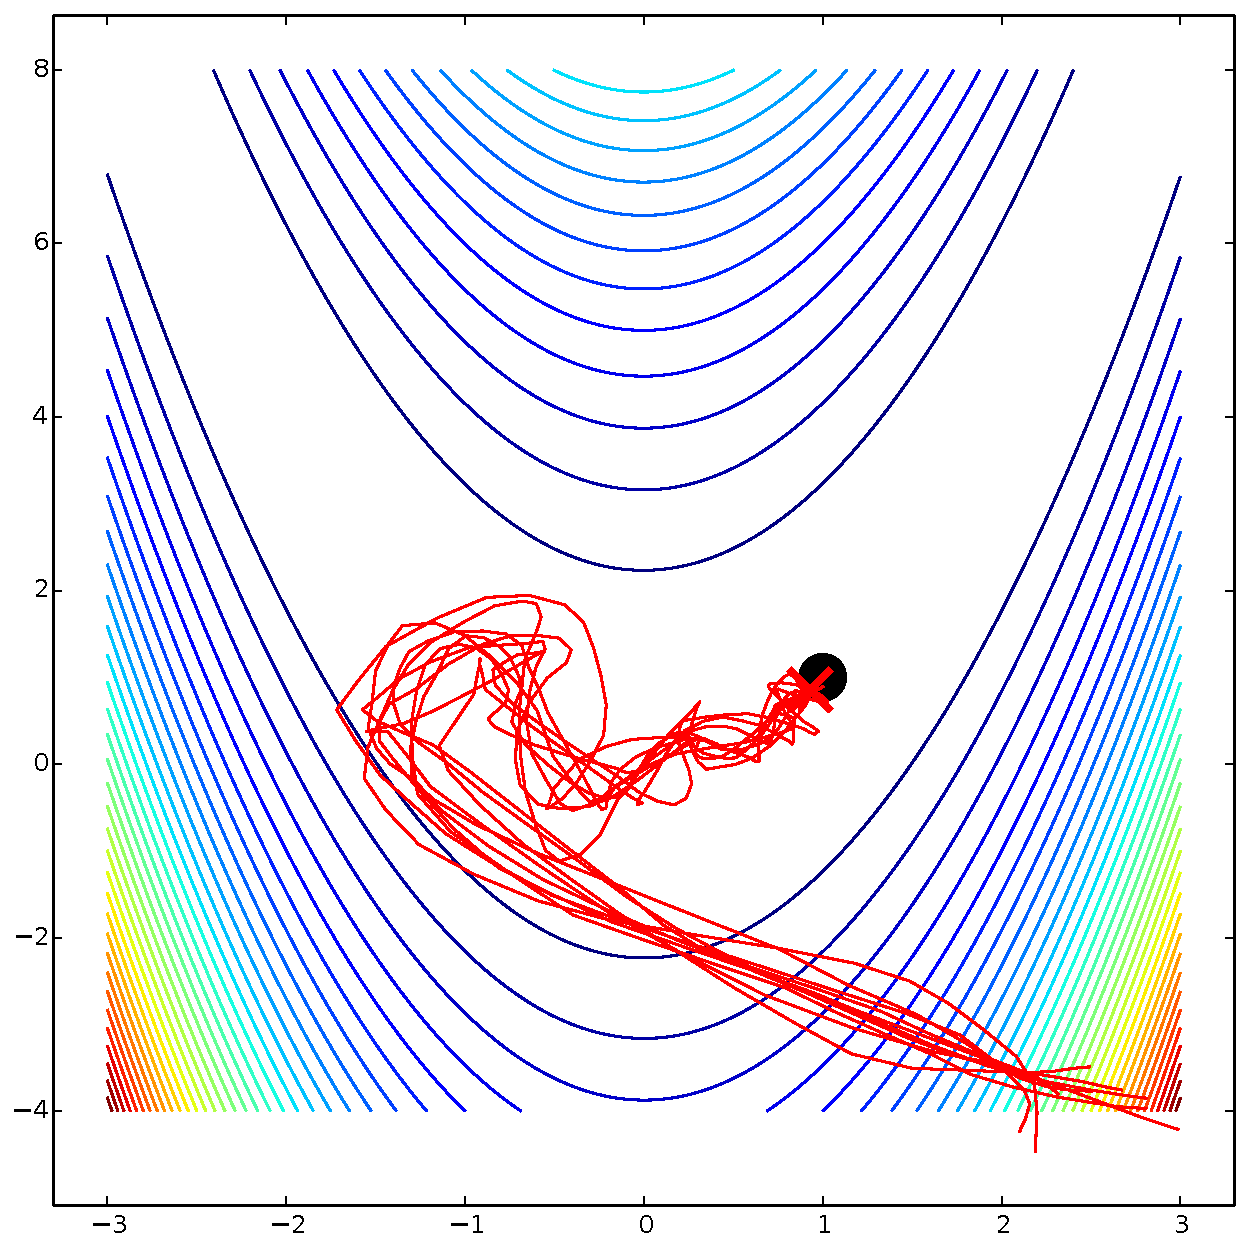
\includegraphics[width=0.45\textwidth]{pso}
    \caption{A particle swarm optimizing the Rosenbrock banana function.}
    \label{fig:pso}
\end{figure}


\subsection{Subfigures}

% if LaTeX (or the margin in your figure file) leads to extra space at
% the top of the page, you may have to reverse the space with something
% like this.  change the -1 to whatever gets you a 1in margin.
% the graduate school is very picky about top margins and sometimes
% vspace is the only solution
\vspace{-1em} 
\begin{figure}[p!]
    \subfloat[The Rosenbrock banana function.]{\label{fig:rosen:banana}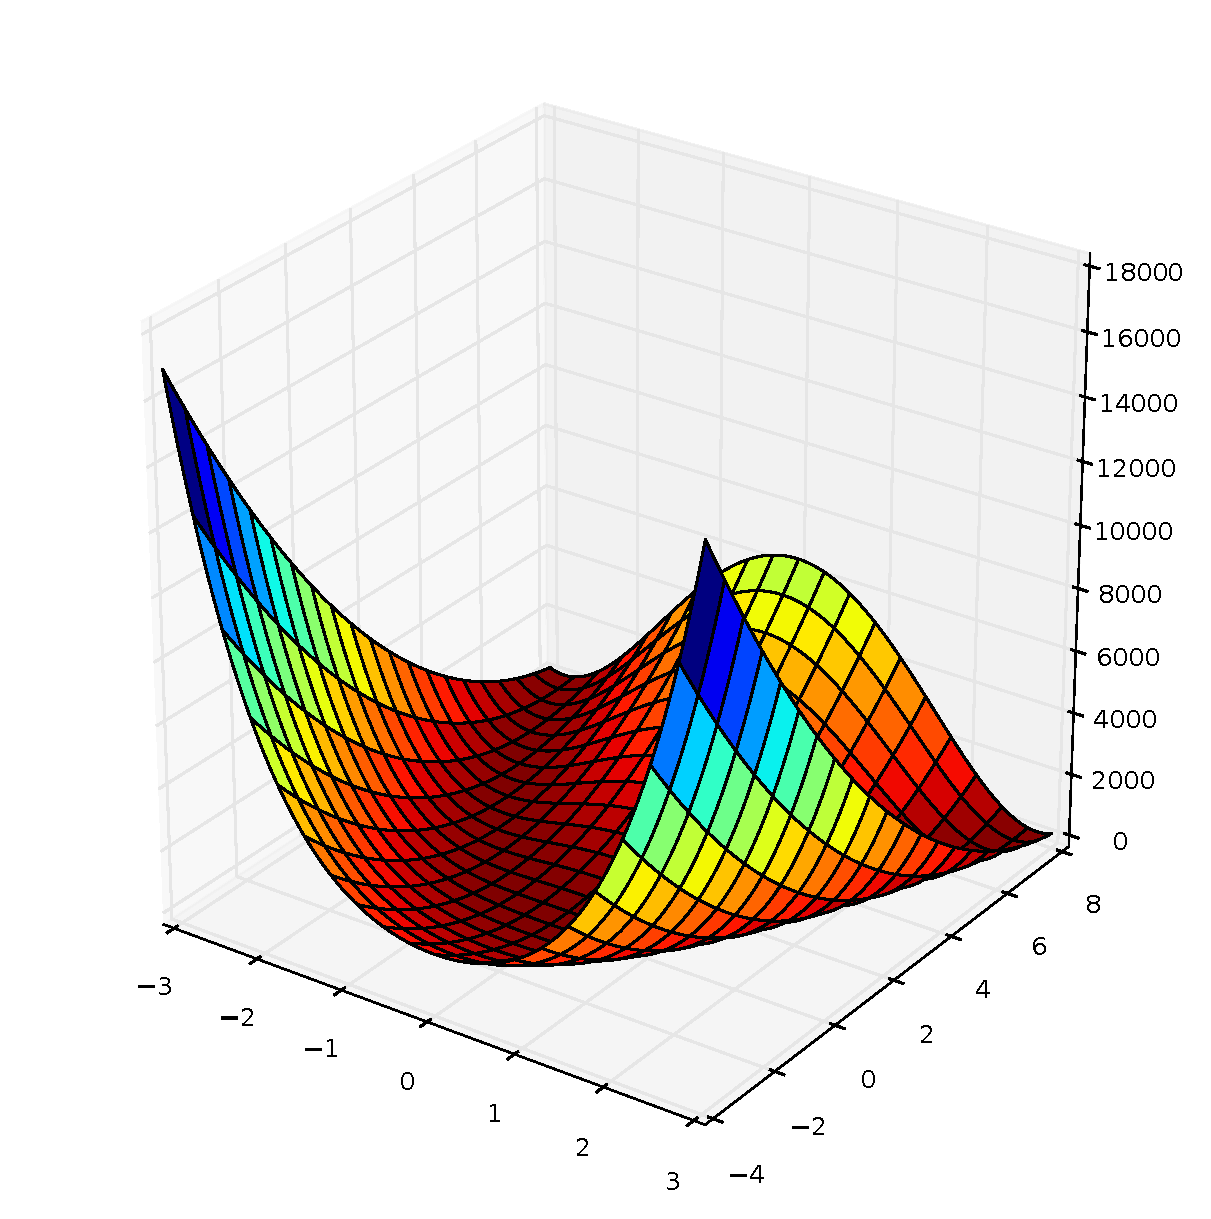
\includegraphics[width=0.45\textwidth]{banana}} \hfill
    \subfloat[Path of the particles.]{\label{fig:rosen:pso}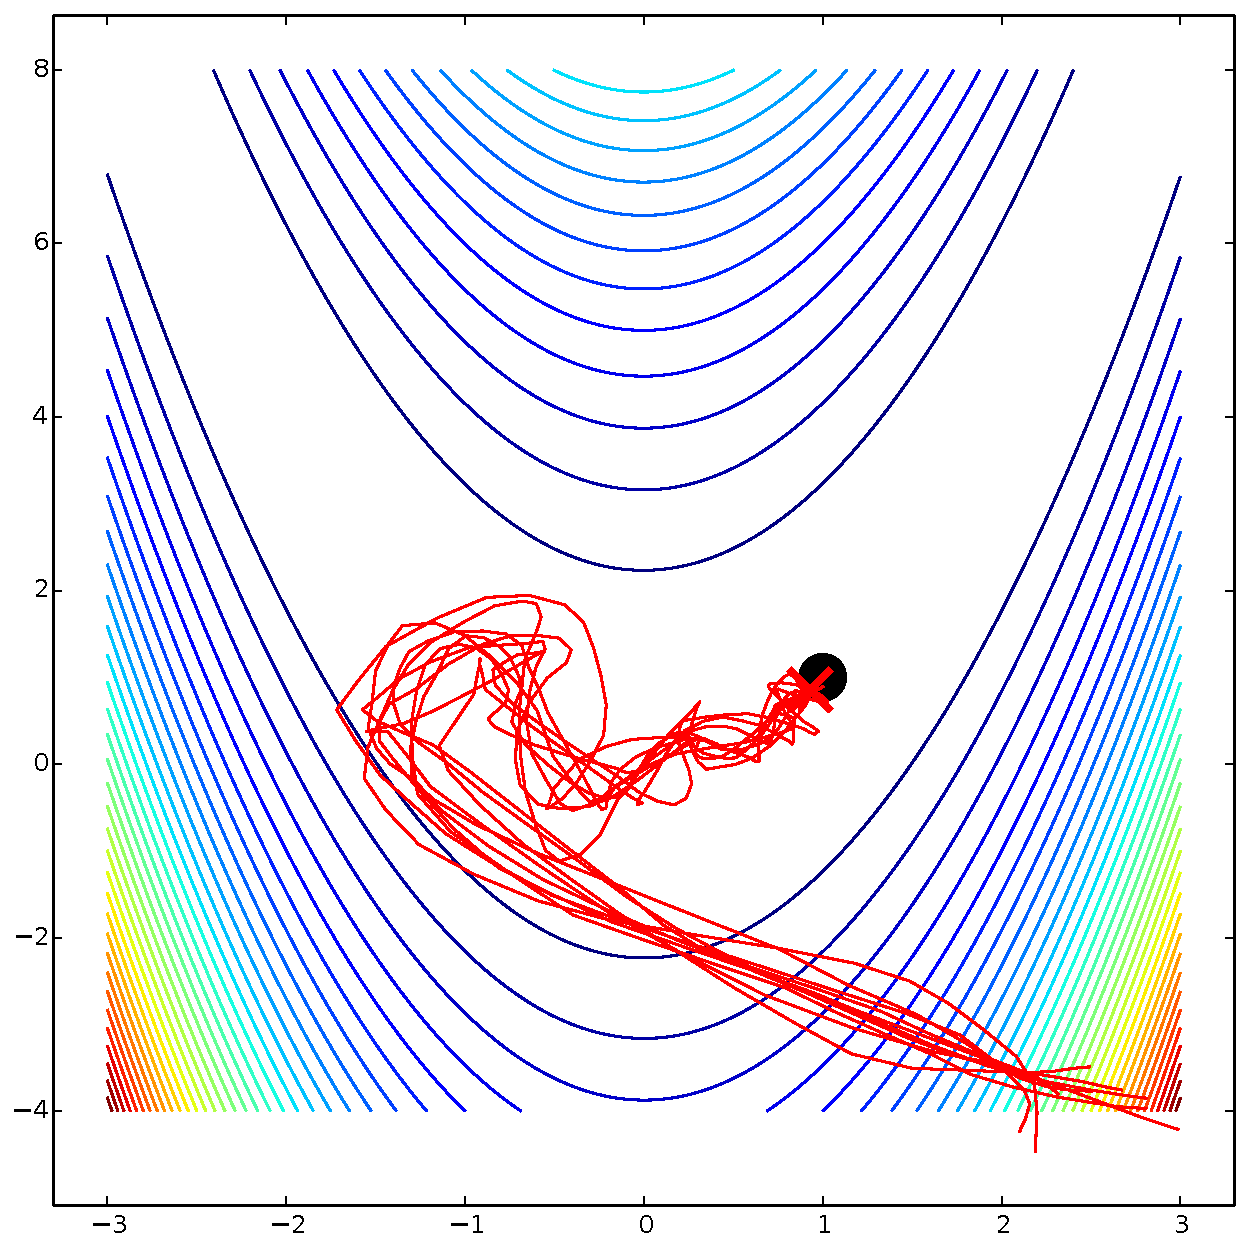
\includegraphics[width=0.45\textwidth]{pso}}
    \caption{Using PSO to optimize the Rosenbrock banana function.  (a)  The function to optimize.  (b)  The path of the particles as they find the global minima.}
\end{figure}

\section{Sideways Pages}

\begin{sidewayspage} % if your figures are too big to fig, things will break
    \vspace{-1em}
    \begin{figure} % don't put [p] here!!
        \subfloat[The Rosenbrock banana function.]{\label{fig:rosen:banana}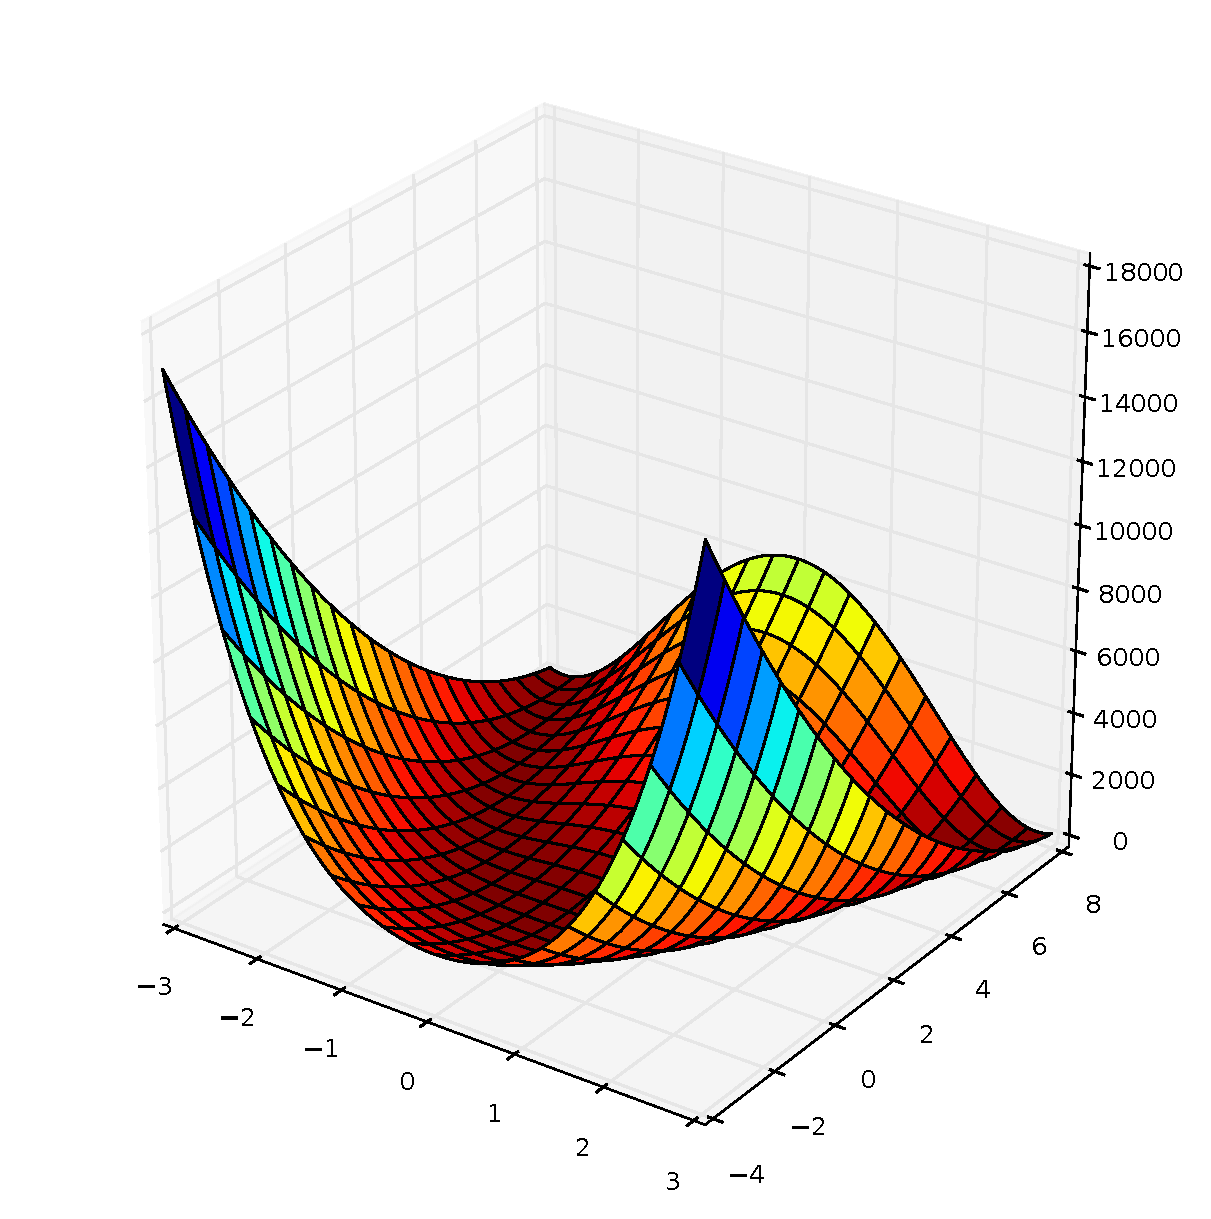
\includegraphics[width=4in]{banana}} \hfill
        \subfloat[Path of the particles.]{\label{fig:rosen:pso}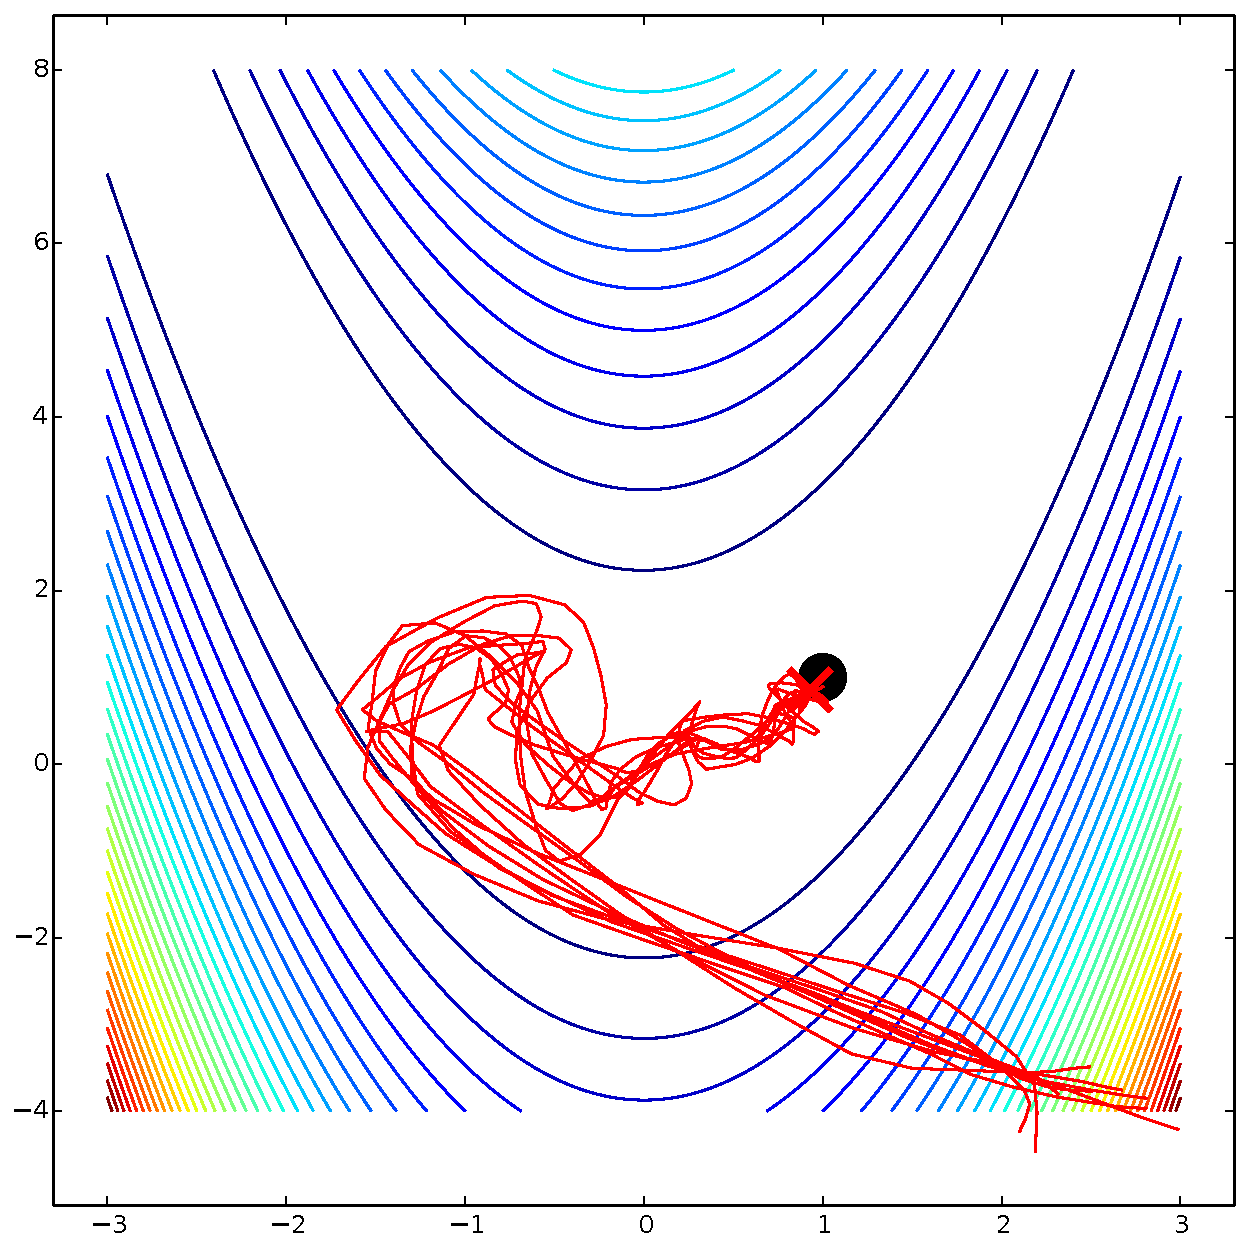
\includegraphics[width=4in]{pso}}
        \caption{Using PSO to optimize the Rosenbrock banana function.  (a)  The function to optimize.  (b)  The path of the particles as they find the global minima.}
    \end{figure}
\end{sidewayspage}

\section{Tables}

\begin{table*}[hp]
    \caption{Sample table.  Caption goes above the table.}
    \label{table:sample}
    \begin{center}
        \begin{tabular}{@{}*{4}{l}} % four columns, left justified
            \toprule
            Data-A  & Data-B    & Data-C    & Data-D \\
            \midrule
            0.5     & 0.5       & 0.5       & 0.5   \\
            0.5     & 0.5       & 0.5       & 0.5   \\
            0.5     & 0.5       & 0.5       & 0.5   \\
            0.5     & 0.5       & 0.5       & 0.5   \\
            0.5     & 0.5       & 0.5       & 0.5   \\
            0.5     & 0.5       & 0.5       & 0.5   \\
            0.5     & 0.5       & 0.5       & 0.5   \\
            0.5     & 0.5       & 0.5       & 0.5   \\
            \midrule
            Mean    & 0.5       & 0.5       & 0.5   \\
            \bottomrule
        \end{tabular}
    \end{center}
\end{table*}

We can reference \tref{table:sample} like this.

\section{Equations}

Equations are the same as they are in most other \LaTeX{} documents.  For example,
\begin{equation}
    \mathbf{z}(t) = \phi(\mathbf{H} \bar{\mathbf{x}}(t) + \mathbf{S} \mathbf{z}(t-1)),
    \label{eq:somefunc}
\end{equation}
where $\mathbf{z}(t)$ is the output of some function at time $t$.  We typically refer to equations as something like \eqref{eq:somefunc}.

\chapter{References}

\section{Citation}

\section{Footnotes}

\section{Bibliography}

Let's cite a bunch of things \cite{forney20112749, cebl, forney2011thesis, forney2015echostate, haykin2009neural}.

\chapter{Formatting Tips and Tricks}

\backmatter % starts unnumbered supplementary material
%%%%%%%%%%%%%%%%%%%%%%%%%%%%%%%%%%%%%%%%%%%%%%%%%%%%%%%%%%%%%%%%

% Bibliography
%%%%%%%%%%%%%%%%%%%%%%%%%%%%%%%%%%%%%%%%%%%%%%%%%%%%%%%%%%%%%%%%

% unsorted BibTeX style
% check here for more:  https://www.sharelatex.com/learn/Bibtex_bibliography_styles
\bibliographystyle{unsrt}
\bibliography{sample} % change readme to the name of your .tex file

\appendix % starts the appendices
%%%%%%%%%%%%%%%%%%%%%%%%%%%%%%%%%%%%%%%%%%%%%%%%%%%%%%%%%%%%%%%%

\chapter{Test Appendix}
\label{appendix:cryptic}
%%%%%%%%%%%%%%%%%%%%%%%%%%%%%%%%%%%%%%%%%%%%%%%%%%%%%%%%%%%%%%%%
\lipsum

% Have a nice day!
%%%%%%%%%%%%%%%%%%%%%%%%%%%%%%%%%%%%%%%%%%%%%%%%%%%%%%%%%%%%%%%%
\end{document}
